\section{Typechecker}
An fs file \textit{TypeChecker.fs} has been implemented, the purpose of which is to ensure that the types, on which arithmetic operators (\textit{plus,minus,etc.}), logical operators (\textit{and,or}) and others, match the given operator.
For example, if we want to implement the \textit{or}-operator, we need to ensure that the operator will only be aplied on boolean values, as any other values don't make sense given the specification of the \textit{or}-operator.\\
The implementation of the typechecker for the \textit{or}-operator, can be seen here: \\
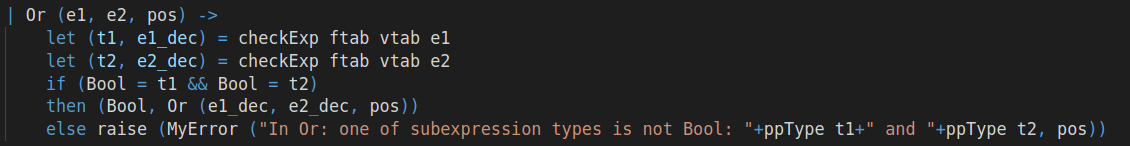
\includegraphics[width=\linewidth]{Materials/TypeChecker/Or}\\
Focusing on the \textit{or}-operator (since other operators are implemented in largely the same way), the typechecking works as follows:\\
First, we call the checkExp function and match with the \textit{Or}-keyword and parse it the two expressions no which we operator and the position.
Afterwards, we determine the type of our expressions by calling the checkExp function whilst supplying it our Function-table and Value-table.\\
Next, we check that both types match (i.e are boolean values). If so, we run theimplemented \textit{or}-function as found in \textit{codeGen.fs} on our expressions, which we now know to be of the type bool. If the \textit{or}-operator is not called on bools, we raise an error stating that at least one of the expressions is of the wrong type.\\
The typechecker works the same for all other operators, except possibly checking on other types like Ints for an arithmetic operator. 
